\documentclass[12pt]{ociamthesis}  % default square logo 
%\documentclass[12pt,beltcrest]{ociamthesis} % use old belt crest logo
%\documentclass[12pt,shieldcrest]{ociamthesis} % use older shield crest logo

%load any additional packages
\usepackage{amssymb}
\usepackage{amsmath}
\usepackage{longtable}
\usepackage{float}


%input macros (i.e. write your own macros file called mymacros.tex 
%and uncomment the next line)
%\include{mymacros}

\title{Program Pendidikan\\[1ex]     %your thesis title,
        Integritas Informatika}   %note \\[1ex] is a line break in the title

\author{
\begin{table}[H]
\centering
\begin{tabular}{ll}
Rolly Maulana Awangga & github.com/awangga          \\
Syafrial Fachri Pane  & github.com/cahyakurniawan   \\
Tri Angga Dio Simamora& github.com/trianggadios		\\
Restiyana Dwi Astuti  & github.com/restiyanada		\\
Dinda Majesty         & github.com/dindamajesty13   \\
\end{tabular}
\end{table}}             %your name
\college{}  %your college

%\renewcommand{\submittedtext}{change the default text here if needed}
\degree{Applied Bachelor Program of Informatics Engineering}     %the degree
\degreedate{Bandung 2019}         %the degree date

%end the preamble and start the document
\begin{document}

%this baselineskip gives sufficient line spacing for an examiner to easily
%markup the thesis with comments
\baselineskip=18pt plus1pt

%set the number of sectioning levels that get number and appear in the contents
\setcounter{secnumdepth}{3}
\setcounter{tocdepth}{3}


\maketitle                  % create a title page from the preamble info
\begin{dedication}
`Jika Kamu tidak dapat menahan lelahnya belajar, \\
Maka kamu harus sanggup menahan perihnya Kebodohan.'\\ 
~Imam Syafi'i~\\
\end{dedication}        % include a dedication.tex file
\begin{acknowledgements}
Pertama-tama kami panjatkan puji dan syukur kepada Allah SWT yang telah memberikan rahmat dan hidayah-Nya sehingga PPK ini dapat diselesaikan.
\end{acknowledgements}   % include an acknowledgements.tex file
\begin{abstract}
Panduan Peningkatan Kompetensi (PPK) ini dibuat dengan tujuan memberikan acuan bagi para sivitas akademika \textit{Informatics Research Center} (IRC) untuk melakukan semua kegiatan yang berada dibawah naungan IRC. Pada intinya PPK menjelaskan secara lengkap tentang standar penilaian setiap kegiatan yang harus dilakukan di IRC. Di dalamnya memuat aturan standar penulisan dan penggunaan Latex sebagai editor. Dengan demikian diharapkan semua sivitas akademika dapat melakukan aktivitas atau kegiatan dengan lancar dan sesuai dengan standar.
\end{abstract}          % include the abstract

\begin{romanpages}          % start roman page numbering
\tableofcontents            % generate and include a table of contents
\listoffigures  
\listoftables            % generate and include a list of figures
\end{romanpages}            % end roman page numbering

%now include the files of latex for each of the chapters etc
\chapter{Tugas Pokok}

Tugas Pokok merupakan pekerjaan yang harus atau wajib dikerjakan selama berada dilingkungan \textit{Informatics Research Center} (IRC). Pelaporan tugas ini wajib dilakukan setiap satu hari sekali dengan menyertakan parameter yang sudah ditentukan yaitu DEDIKASI, PRODUKTIFITAS, INTEGRITAS, DISIPLIN, LOYALITAS, serta KREATIFITAS dan INISIATIF. Untuk penilaian tugas pokok yang sudah di kerjakan satu minggu sebelumnya dilakukan kembali berapa score yang di dapat setiap satu minggu sekali dengan mengakumulasikan dengan poin yang sudah di tentukan terlebih dahulu jumlah pekerjaan per-parameter selama 1 minggu. Poin minimal untuk penilaian mingguan yaitu sebanyak 13 poin. Jika jumlah poin tidak mencapai poin yang sudah di tentukan minimal 13, maka mahasiswa harus menambah pekan untuk mengganti nilai yang kurang tersebut.

\section{Dedikasi}

Menurut KBBI (Kamus besar Bahasa Indonesia), Dedikasi bisa diartikan sebagai suatu pengorbanan tenaga, pikiran, dan waktu yang kita miliki demi keberhasilan suatu usaha atau tujuan yang mulia. Dalam kata lain dedikasi juga bisa diartikan sebagai pengabdian terhadap suatu pekerjaan kita atau tempat kita belajar. Pengabdian atau dedikasi yang bisa dilakukan mahasiswa D4 Teknik Informatika yaitu dengan melakukan pembuatan ataupun pembaharuan modul ajaran yang sudah ada di github atau bisa langsung di lihat di link ini \textbf{\textit{https://github.com/bukuinformatika}}.

Adapun parameter penilaian dedikasi dapat dilihat pada tabel \ref{table:nilaidedikasi}.

\begin{table}[H]
\caption{Penilaian Dedikasi}
\centering
\begin{tabular}{|c|c|c|c|}
\hline
\textbf{No.}&\textbf{Label}&\textbf{Nilai}&\textbf{Keterangan}\\
\hline
1.&TINGGI&3&Full commit selama 5 hari kerja\\
\hline
2.&SEDANG&2&Commit selama 4 hari kerja\\
\hline
3.&RENDAH&1&Commit kurang dari 4 hari kerja\\
\hline
\end{tabular}
\label{table:nilaidedikasi}
\end{table}

\section{Produktifitas}
PProduktivitas merupakan suatu sikap individu dimana kita harus bisa memanejemen waktu dengan baik supaya kita dapat menghasilkan suatu karya atau menghasilkan suatu hal yang bermanfaat bagi diri kita sendiri. Contoh dari pengimplementasian produktivitas misalnya seperti disaat kita melakukan suatu pekerjaan harian pada suatu tempat atau ketika kita sedang melakukan studi, kita harus dapat kita pertanggung jawabkan semua kegiatan yang kita lakukan dalam pekerjaan tersebut.

Adapun parameter penilaian produktifitas dapat dilihat pada tabel \ref{table:nilaiproduktifitas}.

\begin{table}[H]
\caption{Penilaian Produktifitas}
\centering
\begin{tabular}{|c|c|c|c|}
\hline
\textbf{No.}&\textbf{Label}&\textbf{Nilai}&\textbf{Keterangan}\\
\hline
1.&TINGGI&3&Mengerjakan 5 pekerjaan harian\\
\hline
2.&SEDANG&2&Mengerjakan 4 pekerjaan harian\\
\hline
3.&RENDAH&1&Mengerjakan kurang dari 4 pekerjaan harian\\
\hline
\end{tabular}
\label{table:nilaiproduktifitas}
\end{table}

\section{Integritas}
Integritas merupakan salah satu atribut terpenting/kunci yang harus dimiliki seseorang. Dimana integritas ini dapat juga diartikan sebagai syarat untuk kita dimana kita harus/wajib menyelesaikan suatu pekerjaan yang di berikan dengan baik dan tepat waktu, dan didalam integritas ini kita di tuntut untuk meminimalisir kesalah kita dalam suatu pekerjaan.

Adapun parameter penilaian integritas dapat dilihat pada tabel \ref{table:nilaiintegritas}.

\begin{table}[H]
\caption{Penilaian Integritas}
\centering
\begin{tabular}{|c|c|c|c|}
\hline
\textbf{No.}&\textbf{Label}&\textbf{Nilai}&\textbf{Keterangan}\\
\hline
1.&TINGGI&3&Tidak ada penolakan pull request\\
\hline
2.&SEDANG&2&Ada 1 penolakan pull request\\
\hline
3.&RENDAH&1&Ada lebih dari 1 penolakan pull request\\
\hline
\end{tabular}
\label{table:nilaiintegritas}
\end{table}

Catatan:
\begin{itemize}
\item Selesaikan konflik terlebih dahulu, untuk menghindari penolakan saat pull request.
\end{itemize}

\section{Disiplin}
Disiplin merupakan persyaratan yang wajib di ikuti, perasaan taat dan patuh terhadap nilai-nilai yang ada disiplin juga dapat di artika sebagai tanggung jawab terhadap pekerjaan dan waktu yang di berikan. Dengan kata lain disiplin adalah patuh terhadap peraturan yang berlaku
atau tunduk pada pengawasan.

Adapun parameter penilaian disiplin dapat dilihat pada tabel \ref{table:nilaidisiplin}.

\begin{table}[H]
\caption{Penilaian Disiplin}
\centering
\begin{tabular}{|c|c|c|c|}
\hline
\textbf{No.}&\textbf{Label}&\textbf{Nilai}&\textbf{Keterangan}\\
\hline
1.&TINGGI&3&Datang pulang sesuai jadwal selama 5 hari kerja\\
\hline
2.&SEDANG&2&Ada 1 hari terlambat ataupun tidak masuk\\
\hline
3.&RENDAH&1&Ada lebih dari 1 hari terlambat ataupun tidak masuk\\
\hline
\end{tabular}
\label{table:nilaidisiplin}
\end{table}

\section{Loyalitas}
Loyalitas adalah dimana diri kita sendiri dapat melakukan pekerjaan yang menurut kita dapat kita kerjakan tanpa ada paksaan sedikit pun
dengan tulus dan tanpa meminta belas kasihan dari orang lain atau loyalitas dapat di artikan melakukan pekerjaan tanpa meminta imbalan sedikit pun terhadap lingkungan kerja kita.
Contoh dari loyalitas diantaranya:
\begin{enumerate}
\item Menjaga area kerja tetap bersih dan bebas dari debu;
\item Menjaga kerapihan dan kenyaman area kerja;
\item Memperbaiki perangkat kerja yang rusak, dll.
\end{enumerate}
Adapun parameter penilaian loyalitas dapat dilihat pada tabel \ref{table:nilailoyalitas}.

\begin{table}[H]
\caption{Penilaian Loyalitas}
\centering
\begin{tabular}{|c|c|c|c|}
\hline
\textbf{No.}&\textbf{Label}&\textbf{Nilai}&\textbf{Keterangan}\\
\hline
1.&TINGGI&3&Area kerja bersih tanpa debu selama 5 hari kerja\\
\hline
2.&SEDANG&2&Ada 1 hari area kerja tidak bersih\\
\hline
3.&RENDAH&1&Ada lebih dari 1 hari area kerja tidak bersih\\
\hline
\end{tabular}
\label{table:nilailoyalitas}
\end{table}

\section{Kreatif dan Inisiatif}

Adapun parameter penilaian kreatif dan inisiatif dapat dilihat pada tabel ~\ref{table:nilaikreatifinisiatif}.

\begin{table}[H]
\caption{Penilaian Kreatif dan Inisiatif}
\centering
\begin{tabular}{|c|c|c|c|}
\hline
\textbf{No.}&\textbf{Label}&\textbf{Nilai}&\textbf{Keterangan}\\
\hline
1.&TINGGI&3&Menjadi tentor dengan jumlah peserta minimal 10 orang\\
\hline
2.&SEDANG&2&Menjadi tentor dengan jumlah peserta minimal 5 orang\\
\hline
3.&RENDAH&1&Menjadi tentor dengan jumlah peserta kurang dari 5 orang\\
\hline
\end{tabular}
\label{table:nilaikreatifinisiatif}
\end{table}

Catatan:
\begin{enumerate}
\item Kegiatan ini dilaksanakan minimal 1 kali selama Internship atau kegiatan berlangsung, dengan catatan target poin terpenuhi.
\item Target poin yang dicapai minimal 3.
\item Jika poin tidak memenuhi target, maka silahkan untuk mengadakan kegiatan lagi sampai jumlah poin minimal terpenuhi.
\end{enumerate} 
\chapter{Standar Git}
Dari sekian banyaknya git repository GitHub yang paling banyak dipilih\cite{kalliamvakou2014promises} untuk \textit{version-control} agar developer dapat mengetahui atau \textit{tracking} \textit{source-code} yang sedang dibuat. Sebelum melakukan langkah \textit{pull request} alangkah baik anda mempelajari materi \textit{Git} di \textbf{\textit{https://github.com/BukuInformatika/git}} (buka git.pdf).

\section{Standar Git}
Langkah-langkah \textit{pull request} menggunakan \textit{GIT BASH} :
\begin{enumerate}
\item git fetch upstream seperti pada gambar ~\ref{fig:p1}
		\begin{figure}[H]
		\centering
		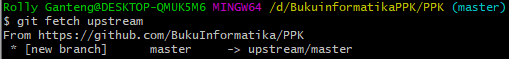
\includegraphics[width=1\textwidth]{figures/pullrequest/p1.PNG}
		\caption{Ini adalah perintah \textit{git fetch upstream}}
		\label{fig:p1}
		\end{figure}
\item git pull upstream master seperti pada gambar \ref{fig:p2}
		\begin{figure}[H]
		\centering
		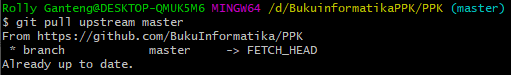
\includegraphics[width=1\textwidth]{figures/pullrequest/p2.PNG}
		\caption{Ini adalah perintah \textit{git pull upstream master}}
		\label{fig:p2}
		\end{figure}
\item edit file yang akan di pull request seperti pada gambar \ref{fig:p3}
		\begin{figure}[H]
		\centering
		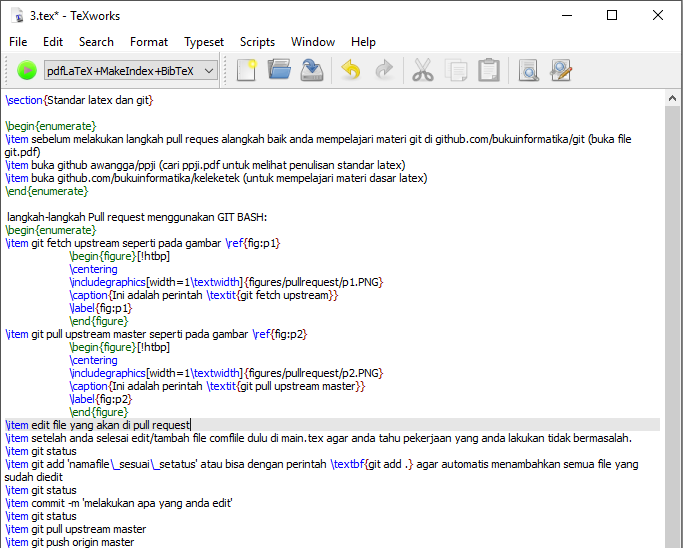
\includegraphics[width=1\textwidth]{figures/pullrequest/p3.PNG}
		\caption{Ini adalah halaman kerja yang siap untuk diedit}
		\label{fig:p3}
		\end{figure}
\item setelah anda selesai edit/tambah file comflile dulu di main.tex agar anda tahu pekerjaan yang anda lakukan tidak bermasalah. dengan memulai compile seperti pada gambar \ref{fig:p4}
		\begin{figure}[H]
		\centering
		
\includegraphics[width=1\textwidth]{figures/pullrequest/p4.PNG}
		\caption{Ini adalah langkah meng-compile}
		\label{fig:p4}
		\end{figure}
\item git status maka kita akan mengetahui apa saja yang belum ditambahkan seperti pada gambar \ref{fig:p5}
		\begin{figure}[H]
		\centering
		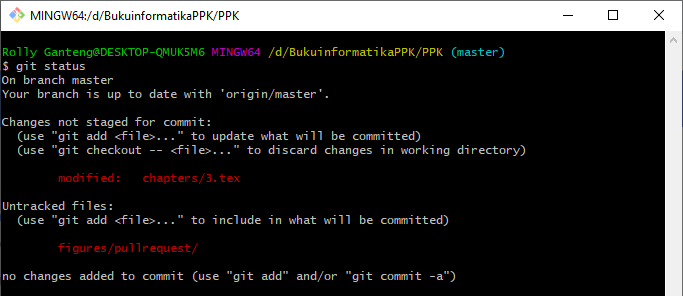
\includegraphics[width=1\textwidth]{figures/pullrequest/p5.PNG}
		\caption{Ini adalah perintah \textit{git status}}
		\label{fig:p5}
		\end{figure}
\item git add 'namafile\_sesuai\_setatus' atau bisa dengan perintah \textbf{git add .} agar automatis menambahkan semua file yang sudah diedit seperti pada gambar \ref{fig:p6}
		\begin{figure}[H]
		\centering
		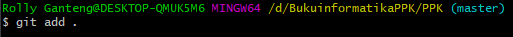
\includegraphics[width=1\textwidth]{figures/pullrequest/p6.PNG}
		\caption{Ini adalah perintah \textit{git add}}
		\label{fig:p6}
		\end{figure}
\item git status seperti pada gambar \ref{fig:p7}
		\begin{figure}[H]
		\centering
		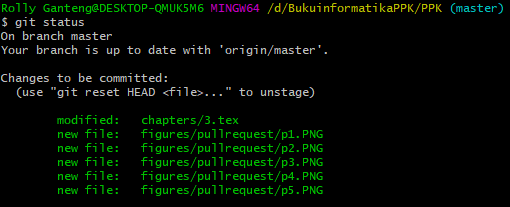
\includegraphics[width=1\textwidth]{figures/pullrequest/p7.PNG}
		\caption{Ini adalah perintah \textit{git status}}
		\label{fig:p7}
		\end{figure}
\item commit -m 'melakukan apa yang anda edit' seperti pada gambar \ref{fig:p8}
		\begin{figure}[H]
		\centering
		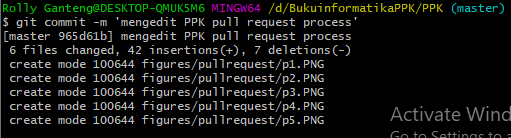
\includegraphics[width=1\textwidth]{figures/pullrequest/p8.PNG}
		\caption{Ini adalah perintah \textit{git commit}}
		\label{fig:p8}
		\end{figure}
\item git pull upstream master
		\begin{figure}[H]
		\centering
		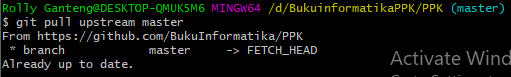
\includegraphics[width=1\textwidth]{figures/pullrequest/p9.PNG}
		\caption{Ini adalah perintah \textit{git pull upstream master}}
		\label{fig:p9}
		\end{figure}
\item git push origin master seperti pada gambar \ref{fig:p10}
		\begin{figure}[H]
		\centering
		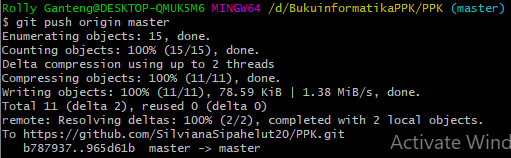
\includegraphics[width=1\textwidth]{figures/pullrequest/p10.PNG}
		\caption{Ini adalah perintah \textit{git push origin master}}
		\label{fig:p10}
		\end{figure}
\end{enumerate}

Buka repositori anda untuk new pull request:
\begin{enumerate}
\item Klik New Pull request pada gambar yang diberi tanda kotak warna merak \ref{labelgambar1}
		\begin{figure}[H]
		\centering
		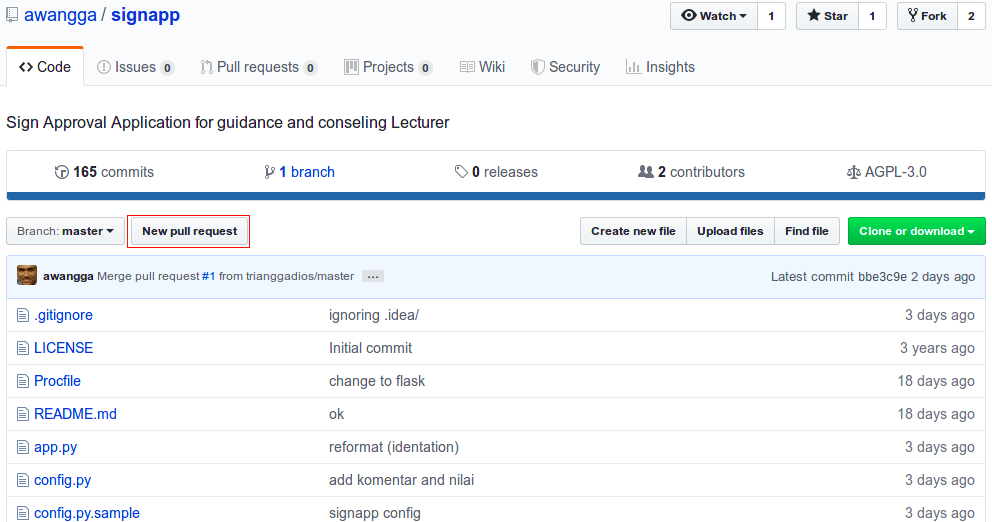
\includegraphics[width=1\textwidth]{figures/1.png}
		\caption{Gambar klik pull request}
		\label{labelgambar1}
		\end{figure}
\item Klik tombol hijau seperti pada gambar lihat tanda yang diberi kotak warna merah \ref{labelgambar2} 
		\begin{figure}[H]
		\centering
		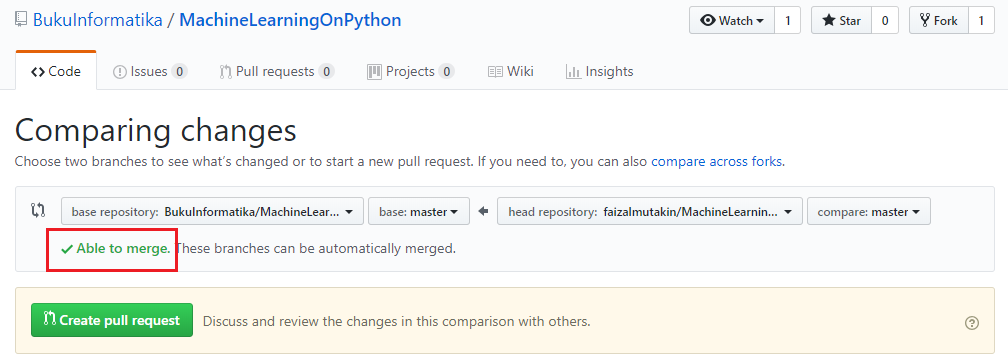
\includegraphics[width=1\textwidth]{figures/2.PNG}
		\caption{Gambar new pull request}
		\label{labelgambar2}
		\end{figure}	 
\end{enumerate}
\chapter{Standar LateX}

Pertama pahami dulu bagaimana bada isi file .tex yang akan kita kerjakan. Download atau lihat salah satu file \textit{LateX} yang akan kita kerjakan. Untuk mengisi \textit{LateX} kita harus mengisinya di dalam komponen yang merupakan \textit{tag} dengan pembuka \textit{begin} dan diakhiri dengan \textit{end}. Kemudian kenali bagian buku terdiri dari \textit{part}, \textit{chapter}, dan \textit{section}. \textit{Part} itu bisa kita andaikan \textit{bab}, \textit{subbab}, \textit{chapter}, dan \textit{section}, adalah bagian.

Kita bisa memisahkan isi dari \textit{LaTeX} dengan perintah input kemudian di dalam kurung kurawal letak file .tex yang akan kita masukkan kedalam file utama \textit{LaTeX} tersebut. \textit{LaTeX} merupakan program pengolahan kata atau sistem persiapan pembuatan dokumen untuk pengetikan sistem \textit{TeX}, yang dinamakan berdasarkan gaya penulisan-nya sebagai \textit{LaTeX}. Nama \textit{LaTeX} itu sendiri hanya mengacu pada bahasa penulisan yang digunakan pada sebuah dokumen, bukan pada editor yang digunakan untuk menulis dokumen tersebut. Untuk membuat dokumen dalam format \textit{LaTeX}, sebuah file berformat .tex harus dibuat menggunakan semacam \textit{text editor}. Walaupun, banyak \textit{text editor} yang dapat digunakan untuk membuat dokumen \textit{LaTeX}, beberapa \textit{text editor} sengaja dibuat khusus untuk menggunakan bahasa \textit{LaTeX}. Untuk panduan lebih lengkap silahkan kunjungi materi di \textbf{\textit{https://github.com/BukuInformatika
/keleketex}}

\section{Hello \textit{LaTeX}}
Ketikkan perintah dibawah ini pada \textit{text editor} anda :
		\begin{figure}[H]
		\centering
		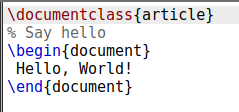
\includegraphics[width=1\textwidth]{figures/hello.png}
		\caption{Gambar hello latex}
		\end{figure}



\chapter{Laporan Harian dan Mingguan}
Laporan harian dan mingguan ini dibuat untuk pengarsipan kegiatan sivitas akademika selama berada dilingkugan \textit{Informatics Research Center} (IRC).

Tujuan pembuatan laporan harian dan mingguan sebagai berikut :
\begin{enumerate}
\item Sebagai informasi individu selama berada dilingkungan IRC
\item Sebagai tolak ukur keaktifan individu selama berada dilingkungan IRC
\item Sebagai penilaian individu terhadap aktivitas yang dilakukan dilingkungan IRC
\end{enumerate}

\section{Contoh Laporan Harian dan Mingguan dengan Tabel}
\begin{table}[H]
\caption{Laporan Harian Tanggal 25 Februari 2018}
\label{tab:lh250219}
\begin{tabular}{|l|l|l|}
\hline
\textbf{No} & \multicolumn{1}{c|}{\textbf{Kategori}} & \multicolumn{1}{c|}{\textbf{Keterangan}} \\ \hline
1 & Dedikasi & - \\ \hline
2 & Produktifitas & \begin{tabular}[c]{@{}l@{}}a. Membuat repositori Modul Praktikum kelas Pemrograman III\\     Kelas 2A, 2B, dan 2C di organisasi pemograman-iii.\end{tabular} \\
 &  & b. Mengintal python, pip, anaconda, dan jupiter dari Udemy. \\
 &  & \begin{tabular}[c]{@{}l@{}}c. Melakukan merge pull request di pemograman-iii/praktikum\_2a,\\    dari \#1, \#3, \#4, \#7, \#8, \#9, \#10, \#12, \#13, dan \#14.\end{tabular} \\ \hline
3 & Integritas & able to merge/has no conflict \\ \hline
4 & Disiplin & Jam Datang : 07.07 WIB \\
 &  & Jam Pulang : 16.20 WIB \\ \hline
5 & Loyalitas & \begin{tabular}[c]{@{}l@{}}Membersihkan dan merapihkan meja kerja, dan mengecek AC\\ di pagi dan sore hari.\end{tabular} \\ \hline
\end{tabular}
\end{table}

% Please add the following required packages to your document preamble:
% \usepackage[normalem]{ulem}
% \useunder{\uline}{\ul}{}
\begin{table}[H]
\caption{Laporan Harian Tanggal 26 Februari 2018}
\label{tab:lh260219}
\begin{tabular}{|l|l|l|}
\hline
\textbf{No} & \multicolumn{1}{c|}{\textbf{Kategori}} & \multicolumn{1}{c|}{\textbf{Keterangan}} \\ \hline
1 & Dedikasi & - \\ \hline
2 & Produktifitas & a. Membuat repositori Modul Praktikum kelas Kecerdasan Buatan. \\
 &  & b. Mendata dan menilai tugas 1 kelas 2A-Pemrograman III. \\
 &  & \begin{tabular}[c]{@{}l@{}}c. Membimbing Fadila, Lusia, dan Rahmi Roza kelas 3C untuk \\     tugas Kecerdasan Buatan.\end{tabular} \\ \hline
3 & Integritas & able to merge/has no conflict \\ \hline
4 & Disiplin & Jam Datang : 08.30 WIB \\
 &  & Jam Pulang : 16.30 WIB \\ \hline
5 & Loyalitas & \begin{tabular}[c]{@{}l@{}}Membersihkan dan merapihkan meja kerja, dan mengecek AC\\ di pagi dan sore hari.\end{tabular} \\ \hline
\end{tabular}
\end{table}

\begin{table}[H]
\caption{Laporan Harian Tanggal 27 Februari 2019}
\label{tab:lh270219}
\begin{tabular}{|l|l|l|}
\hline
\textbf{No} & \multicolumn{1}{c|}{\textbf{Kategori}} & \multicolumn{1}{c|}{\textbf{Keterangan}} \\ \hline
1 & Dedikasi & bukuinformatika/flask \#10 \\ \hline
2 & Produktifitas & a.Mendata dan menilai tugas kelas 3C-Kecerdasan Buatan. \\
 &  & b.Membimbing anak kelas 3C untuk tugas Kecerdasan Buatan. \\
 &  & c. Mengkoordinasi tugas kontribusi anak kelas. \\ \hline
3 & Integritas & able to merge/has no conflict \\ \hline
4 & Disiplin & Jam Datang : 08.50 WIB \\
 &  & Jam Pulang : 17.30 WIB \\ \hline
5 & Loyalitas & \begin{tabular}[c]{@{}l@{}}Membersihkan dan merapihkan meja kerja, dan mengecek AC\\ di pagi dan sore hari.\end{tabular} \\ \hline
\end{tabular}
\end{table}

\begin{table}[H]
\caption{Laporan Harian Tanggal 28 Februari 2019}
\label{tab:lh280219}
\begin{tabular}{|l|l|l|}
\hline
\textbf{No} & \multicolumn{1}{c|}{\textbf{Kategori}} & \multicolumn{1}{c|}{\textbf{Keterangan}} \\ \hline
1 & Dedikasi & BukuInformatika/flask \#12 \\ \hline
2 & Produktifitas & \begin{tabular}[c]{@{}l@{}}a. Evaluasi mingguan dan sosialisasi format baru penilaian peserta\\     internship II di IRC dan Prodi.\end{tabular} \\
 &  & \begin{tabular}[c]{@{}l@{}}b. Memeriksa lembar jawaban UAS GIS kelas 3C dan Arkom\\     kelas 1C.\end{tabular} \\
 &  & c. Menginput nilai UAS kelas 1C, 3A, 3B, dan 3C di google docs. \\
 &  & \begin{tabular}[c]{@{}l@{}}d. Mengkoordinir mahasiswa untuk tugas kontribusi pembuatan cover,\\     pencetakan, sampai pendistribusian buku di Grup Whatsapp.\end{tabular} \\
 &  & \begin{tabular}[c]{@{}l@{}}e. Memeriksa tugas kecerdasan buatan kelas 3C serta menginput nilai\\     ke google docs atas nama Fadila, Lusia Violita Aprilian, dan Rahmi.\end{tabular} \\ \hline
3 & Integritas & able to merge/has no conflict \\ \hline
4 & Disiplin & Jam Datang : 07.55 WIB \\
 &  & Jam Pulang : 17.00 WIB \\ \hline
5 & Loyalitas & \begin{tabular}[c]{@{}l@{}}Menyapu, membersihkan dan merapihkan meja, mencuci gelas nomor 6,\\ dan mengecek AC di pagi dan sore hari.\end{tabular} \\ \hline
\end{tabular}
\end{table}

\begin{table}[H]
\caption{Laporan Harian Tanggal 1 Maret 2019}
\label{tab:lh010319}
\begin{tabular}{|l|l|l|}
\hline
\textbf{No} & \multicolumn{1}{c|}{\textbf{Kategori}} & \multicolumn{1}{c|}{\textbf{Keterangan}} \\ \hline
1 & Dedikasi &  \\ \hline
2 & Produktifitas & \begin{tabular}[c]{@{}l@{}}a. Mengerjakan Soal Toefl Pre-Test 2 (Computer Based)\\     Skor Toefl: 55\end{tabular} \\
 &  & b. Mendata skor toefl peserta Internship II di IRC. \\
 &  & c. Memeriksa pull request di laporanirc/2019. \\ \hline
3 & Integritas & able to merge/has no conflict \\ \hline
4 & Disiplin & Jam Datang : 07.39 WIB \\
 &  & Jam Pulang : 14.20 WIB \\ \hline
5 & Loyalitas & \begin{tabular}[c]{@{}l@{}}Menyapu, membersihkan dan merapihkan meja, membeli\\ sabun dan spons cuci piring, dan mengecek AC di pagi\\ dan sore hari.\end{tabular} \\ \hline
\end{tabular}
\end{table}

\section{Penilaian Mingguan (Tabel)}
Penilaian mingguan ini dilakukan setiap hari Jum'at, penilain ini akumulasi dari total laporan harian.

\begin{table}[H]
\centering
\caption{Nilai Minggu ke-1}
\label{tab:nm01}
\begin{tabular}{|c|c|c|}
\hline
\textbf{No} & \textbf{Kategori} & \textbf{Poin} \\ \hline
1 & Dedikasi & 1 \\ \hline
2 & Produktifitas & 3 \\ \hline
3 & Integritas & 3 \\ \hline
4 & Disiplin & 3 \\ \hline
5 & Loyalitas & 3 \\ \hline
 & \textbf{Total Poin} & 13 \\ \hline
\end{tabular}
\end{table}

\section{Contoh Laporan Harian dan Mingguan dengan Penomoran}

\begin{enumerate}
\item \textbf{Tugas Harian tanggal 17/01/2019}
\begin{enumerate}
\item Membersihkan ruang IRC
\item Diskusi mengenai penataan ulang ruang IRC
\end{enumerate}

\item \textbf{Tugas Harian tanggal 18/01/2019}
\begin{enumerate}
\item Membersihkan ruang IRC
\item Diskusi mengenai rancangan ruang IRC
\item Diskusi mengenai barang yang harus ditambahkan di ruang IRC
\item Membuat artikel untuk bahan majalah D4 TI
\end{enumerate}

\item \textbf{Tugas Harian tanggal 21/01/2019}
\begin{enumerate}
\item Mencari artikel untuk bahan majalah
\item Diskusi tentang perancangan ruang sidang di IRC
\end{enumerate}

\item \textbf{Tugas Harian tanggal 30/02/2019}
\begin{enumerate}
\item Mendata buku yang akan dipindahkan ke IRC
\end{enumerate}

\item \textbf{Tugas Harian tanggal 31/01/2019}
\begin{enumerate}
\item Memberi label pada buku untuk IRC
\item Memindahkan buku sumbangan ke IRC
\end{enumerate}

\item \textbf{Tugas Harian tanggal 01/02/2019}
\begin{enumerate}
\item Praktek github dengan Pak Rolly Maulana Awangga 
\end{enumerate}

\item \textbf{Tugas Harian tanggal 06/02/2019}
\begin{enumerate}
\item Membuat video pesan, kesan dan kritik untuk IRC
\end{enumerate}

\item \textbf{Tugas Harian tanggal 18/02/2019}
\begin{enumerate}
\item Memperhatikan tingkat 3 presentasi
\item Mengoreksi laporan tingkat 3 yang presentasi
\item Memeriksa revisian tutorial class diagram adik tingkat
\end{enumerate}

\item \textbf{Tugas Harian tanggal 25/02/2019}
\begin{enumerate}
\item Masuk Kelas Pemrograman III
\item Menginstal python, anaconda
\item Menambah materi udemy (commit 8b5991b08ef04a0c1581f5976017e7eab865c856)
\item Menambah materi di GIS2019 (commit f1535f03dd64c09ddba50f68371ec04b878846e9, commit 0ff764471c1cefd7e6b20d81027d7d810c1343d5, commit c054dcbfa03e9a2d9ef56f3302d8f0854840d758)
\item Memeriksa tugas Pemrograman III kelas 2b (1174034 Ichsan Hizman Hardy, 1174050 Dika Sukma Pradana, 1174042 Faisal Najib Abdullah, 1174035 Luthfi Muhammad Nabil, 1174040 Hagan Rowlenstino, 1174043 Irvan Rizkiansyah, 1174063 Muhamad Iqbal Panggabean, 1174057 Alit fajar Kurniawan, 1174059 Kevin Natanael Nainggolan)
\end{enumerate}

\textbf{Dedikasi}
\begin{enumerate} 
\item  Menambah materi di GIS2019 (commit f1535f03dd64c09ddba50f68371ec04b878846e9, commit 0ff764471c1cefd7e6b20d81027d7d810c1343d5, commit c054dcbfa03e9a2d9ef56f3302d8f0854840d758)
\end{enumerate}

\textbf{Produktifitas}
\begin{enumerate}
\item Masuk Kelas Pemrograman III
\item Menginstal python, anaconda
\item Menambah materi udemy (commit 8b5991b08ef04a0c1581f5976017e7eab865c856
\item Menambah materi di GIS2019 (commit f1535f03dd64c09ddba50f68371ec04b878846e9, commit 0ff764471c1cefd7e6b20d81027d7d810c1343d5, commit c054dcbfa03e9a2d9ef56f3302d8f0854840d758)
\item Memeriksa tugas Pemrograman III kelas 2b (1174034 Ichsan Hizman Hardy, 1174050 Dika Sukma Pradana, 1174042 Faisal Najib Abdullah, 1174035 Luthfi Muhammad Nabil, 1174040 Hagan Rowlenstino, 1174043 Irvan Rizkiansyah, 1174063 Muhamad Iqbal Panggabean, 1174057 Alit fajar Kurniawan, 1174059 Kevin Natanael Nainggolan)
\end{enumerate}

\textbf{Integritas}
\begin{enumerate}
\item able to merge/has no conflict
\end{enumerate}

\textbf{Disiplin}
\begin{enumerate}
\item Jam Masuk : 08.40
\item Jam Keluar : 15.30
\end{enumerate}

\textbf{Loyalitas}
\begin{enumerate}
\item Mengecek AC saat datang dan pulang dari IRC
\item Merapihkan meja dan kursi saat pulang dari IRC
\item Merapihkan CPU ke lemari
\item Merapihkan banner ke lemari
\item Menjaga peralatan yang ada di IRC  
\end{enumerate}

\item \textbf{Tugas Harian tanggal 26/02/2019}
\begin{enumerate}
\item Masuk kelas Kecerdasan Buatan
\item Membuat repository tugas kecerdasan buatan kelas 3c
\item Menginput nilai tugas Pemrograman III kelas 2b
\item Menambah materi GIS 2019, commit d97e9474087a3faca296fef82e9e7503345ac45e
\end{enumerate}

\textbf{Dedikasi}
\begin{enumerate}
\item Menambah materi GIS 2019, commit d97e9474087a3faca296fef82e9e7503345ac45e
\end{enumerate}

\textbf{Produktifitas}
\begin{enumerate}
\item Masuk kelas Kecerdasan Buatan
\item Membuat repository tugas kecerdasan buatan kelas 3c
\item Menginput nilai tugas Pemrograman III kelas 2b
\item Menambah materi GIS 2019, commit d97e9474087a3faca296fef82e9e7503345ac45e
\end{enumerate}

\textbf{Integritas}
\begin{enumerate}
\item able to merge/has no conflict
\end{enumerate}

\textbf{Disiplin}
\begin{enumerate}
\item Jam Masuk : 08.40
\item Jam Keluar : 15.30
\end{enumerate}

\textbf{Loyalitas}
\begin{enumerate}
\item Mengecek AC saat datang dan pulang dari IRC
\item Merapihkan kursi saat pulang dari IRC
\item Menjaga peralatan yang ada di IRC
\end{enumerate}

\item \textbf{Tugas Harian tanggal 27/02/2019}
\begin{enumerate}
\item Mangecek tugas kecerdasan buatan kelas 3c
\item Menginput nilai tugas kecerdasan buatan kelas 3c
\item Memberikan arahan dan hukuman bagi mahasiswa yang tidak melakukan pull request, tidak membenarkan conflict dan tidak mengerjakan tugas Pemrograman III kelas 2b
\item Menginput nilai tugas Pemrograman III kelas 2b (1174034 Ichsan Hizman Hardy, 1174050 Dika Sukma Pradana, 1174042 Faisal Najib Abdullah, 1174035 Luthfi Muhammad Nabil, 1174040 Hagan Rowlenstino, 1174043 Irvan Rizkiansyah, 1174063 Muhamad Iqbal Panggabean, 1174057 Alit fajar Kurniawan, 1174059 Kevin Natanael Nainggolan)
\item Menambah materi GIS 2019, commit d97e9474087a3faca296fef82e9e7503345ac45e
\item Menandatangani acc tutorial membuat class diagram (Ajis Trigunawan 1164031 dan Wildan Khaustara W 1164058)
\item Memeriksa dan memberi revisian jurnal projek II Ajis Trigunawan 1164031
\end{enumerate}

\textbf{Dedikasi}
\begin{enumerate}
\item Menambah materi GIS 2019, commit d97e9474087a3faca296fef82e9e7503345ac45e
\end{enumerate}

\textbf{Produktifitas}
\begin{enumerate}
\item Masuk kelas Kecerdasan Buatan
\item Membuat repository tugas kecerdasan buatan kelas 3c
\item Menginput nilai tugas Pemrograman III kelas 2b (1174034 Ichsan Hizman Hardy, 1174050 Dika Sukma Pradana, 1174042 Faisal Najib Abdullah, 1174035 Luthfi Muhammad Nabil, 1174040 Hagan Rowlenstino, 1174043 Irvan Rizkiansyah, 1174063 Muhamad Iqbal Panggabean, 1174057 Alit fajar Kurniawan, 1174059 Kevin Natanael Nainggolan)
\item Menambah materi GIS 2019, commit d97e9474087a3faca296fef82e9e7503345ac45e
\item Menandatangani acc tutorial membuat class diagram (Ajis Trigunawan 1164031 dan Wildan Khaustara W 1164058)
\item Memeriksa dan memberi revisian jurnal projek II Ajis Trigunawan 1164031
\end{enumerate}

\textbf{Integritas}
\begin{enumerate}
\item able to merge/has no conflict
\end{enumerate}

\textbf{Disiplin}
\begin{enumerate}
\item Jam Masuk : 08.40
\item Jam Keluar : 15.30
\end{enumerate}

\textbf{Loyalitas}
\begin{enumerate}
\item Mengecek AC saat datang dan pulang dari IRC
\item Merapihkan kursi saat pulang dari IRC
\item Menjaga peralatan yang ada di IRC
\end{enumerate}

\item \textbf{Tugas Harian tanggal 27/02/2019}
\begin{enumerate}
\item Mangecek tugas kecerdasan buatan kelas 3c (Andi Muh Aslam 1164064 dan Aip Suprapto Munari 1164063)
\item Menginput nilai tugas kecerdasan buatan kelas 3c (Andi Muh Aslam 1164064 dan Aip Suprapto Munari 1164063)
\item Memberikan arahan dan hukuman bagi mahasiswa yang tidak melakukan pull request, tidak membenarkan conflict dan tidak mengerjakan tugas Pemrograman III kelas 2b
\item Menambah gambar pada Materi GIS (menambahkan gambar \#11) 
\end{enumerate}

\textbf{Dedikasi}
\begin{enumerate}
\item Menambah gambar pada Materi GIS (menambahkan gambar \#11) 
\end{enumerate}

\textbf{Produktifitas}
\begin{enumerate}
\item Mangecek tugas kecerdasan buatan kelas 3c (Andi Muh Aslam 1164064 dan Aip Suprapto Munari 1164063)
\item Menginput nilai tugas kecerdasan buatan kelas 3c (Andi Muh Aslam 1164064 dan Aip Suprapto Munari 1164063)
\item Memberikan arahan dan hukuman bagi mahasiswa yang tidak melakukan pull request, tidak membenarkan conflict dan tidak mengerjakan tugas Pemrograman III kelas 2b
\item Menambah gambar pada Materi GIS (menambahkan gambar \#11) 
\end{enumerate}

\textbf{Integritas}
\begin{enumerate}
\item able to merge/has no conflict
\end{enumerate}

\textbf{Disiplin}
\begin{enumerate}
\item Jam Masuk : 08.40
\item Jam Keluar : 15.30
\end{enumerate}

\textbf{Loyalitas}
\begin{enumerate}
\item Mengecek AC saat datang dan pulang dari IRC
\item Merapihkan kursi saat pulang dari IRC
\item Menjaga peralatan yang ada di IRC
\end{enumerate}


\item \textbf{Tugas Harian tanggal 28/02/2019}
\begin{enumerate}
\item Evaluasi mingguan dengan Pak Rolly Maulana Awangga
\item Menilai hasil UAS kelas 1C, 3A dan 3C
\item Menata ulang ruang IRC
\item Memeriksa tugas kelas Kecerdasan Buatan 3C Andi Muh Aslam 1164064, hari2 \#3 dan  Aip Suprapto Munari 1164063  (tugas masih conflict)
\item Menginput nilai tugas Kecerdasan Buatan kelas 3C Andi Muh Aslam 1164064 dan Aip Suprapto Munari 1164063 
\item Menambah materi sumber sumber data geospasial \#13
\end{enumerate}

\textbf{Dedikasi}
\begin{enumerate}
\item Menambah materi sumber sumber data geospasial \#13
\end{enumerate}

\textbf{Produktifitas}
\begin{enumerate}
\item Evaluasi mingguan dengan Pak Rolly Maulana Awangga
\item Menilai hasil UAS kelas 1C, 3A dan 3C
\item Menata ulang ruang IRC
\item Memeriksa tugas kelas Kecerdasan Buatan 3C Andi Muh Aslam 1164064, hari2 \#3 dan  Aip Suprapto Munari 1164063  (tugas masih conflict)
\item Menginput nilai tugas Kecerdasan Buatan kelas 3C Andi Muh Aslam 1164064 dan Aip Suprapto Munari 1164063 
\end{enumerate}

\textbf{Integritas}
\begin{enumerate}
\item able to merge/has no conflict
\end{enumerate}

\textbf{Disiplin}
\begin{enumerate}
\item Jam Masuk : 08.40
\item Jam Keluar : 17.30
\end{enumerate}

\textbf{Loyalitas}
\begin{enumerate}
\item Mengecek AC saat datang dan pulang dari IRC
\item Merapihkan kursi saat pulang dari IRC
\item Menjaga peralatan yang ada di IRC
\item Mengatur ulang ruang IRC 
\end{enumerate}

\item \textbf{Tugas Harian tanggal 01/03/2019}
\begin{enumerate} 
\item Melakukan pre test TOEFL 
\item Memberi tahu kelas 3B untuk mencantumkan sitasi dan sumber di daftar pustaka mengenai materi GIS
\item menambah materi dan gambar mengenai sumber sumber data geospasial \#16
\end{enumerate}

\textbf{Dedikasi}
\begin{enumerate}
\item menambah materi dan gambar mengenai sumber sumber data geospasial \#16
\end{enumerate}

\textbf{Produktifitas}
\begin{enumerate}
\item Melakukan pre test TOEFL 
\item Memberi tahu kelas 3B untuk mencantumkan sitasi dan sumber di daftar pustaka mengenai materi GIS
\item menambah materi dan gambar mengenai sumber sumber data geospasial \#16
\end{enumerate}

\textbf{Integritas}
\begin{enumerate}
\item able to merge/has no conflict
\end{enumerate}


\textbf{Disiplin}
\begin{enumerate}
\item Jam Masuk : 08.40
\item Jam Keluar : 11.40 (Dikarenakan ada sosialisasi INTERNSHIP II)
\end{enumerate}


\textbf{Loyalitas}
\begin{enumerate}
\item Mengecek AC saat datang dan pulang dari IRC
\item Menjaga peralatan yang ada di IRC
\item Merapihkan kursi setelah pulamg dari IRC
\item Mengelap meja pribadi
\item Menyapu dan merapihkan area sidang IRC
\item Membersihkan lemari buku 
\end{enumerate}

\item \textbf{Tugas Harian tanggal 04/03/2019}
\begin{enumerate}
\item Menambah gambar dan materi mengenai sumber sumber data geospasial \#17
\item Masuk kelas Pemrograman 3 
\item Diskusi mengenai INTERNSHIP II bersama Bapak Rolly Maulana Awangga
\item Membuat orgnanisasi INTERNSHIPD4TI di github
\item Kontribusi pada repository PPK (template \#1, merapihkan dan menambah contoh laporan harian dan mingguan \#8)
\item Menambah materi deep learning computer vision \#3
\item Membersihkan meja pribadi
\item Membersihkan area sidang 
\end{enumerate}

\textbf{Dedikasi}
\begin{enumerate}
\item Menambah gambar dan materi mengenai sumber sumber data geospasial \#17
\item Kontribusi pada repository PPK (template \#1, merapihkan dan menambah contoh laporan harian dan mingguan \#8)
\item Menambah materi deep learning computer vision \#3
\end{enumerate}

\textbf{Produktifitas}
\begin{enumerate}
\item Menambah gambar dan materi mengenai sumber sumber data geospasial \#17
\item Masuk kelas Pemrograman 3 
\item Diskusi mengenai INTERNSHIP II bersama Bapak Rolly Maulana Awangga
\item Membuat orgnanisasi INTERNSHIPD4TI di github
\item Kontribusi pada repository PPK (template \#1, merapihkan dan menambah contoh laporan harian dan mingguan \#8)
\item Menambah materi deep learning computer vision \#3
\item Membersihkan meja pribadi
\item Menyapu dan merapihkan area sidang 
\end{enumerate}

\textbf{Integritas}
\begin{enumerate}
\item able to merge/has no conflict
\end{enumerate}


\textbf{Disiplin}
\begin{enumerate}
\item Jam Masuk : 08.40
\item Jam Keluar : 17.40
\end{enumerate}


\textbf{Loyalitas}
\begin{enumerate}
\item Mengecek AC saat datang dan pulang dari IRC
\item Menjaga peralatan yang ada di IRC
\item Merapihkan kursi setelah pulamg dari IRC
\item Mengelap meja pribadi
\item Menyapu dan merapihkan area sidang IRC
\item Membersihkan meja pribadi
\end{enumerate}
\end{enumerate}

\section{Penilaian Mingguan (Penomoran)}
Total score mingguan adalah 15 keterangan seperti pada Tabel ~\ref{table:scoremingguan}.
\begin{table}[H]
\centering
\begin{tabular}{ |c|c|c|c|c|c|c|c|c|c| }
\hline
Kategori & Keterangan Nilai \\
\hline
Dedikasi & 3 \\
\hline
Produktif & 3 \\
\hline
Integritas & 3 \\
\hline
Disiplin & 3 \\
\hline
Loyalitas & 3 \\
\hline
\end{tabular}
\caption{Tabel Score Mingguan}
\label{table:scoremingguan}
\end{table}
\chapter{E-Sertifikat}

\section{e-Sertifikat}
Setelah semua parameter standar penilaian telah selesai dan sudah terpenuhi. \textit{Informatics Research Center} akan mengeluarkan e-Sertifikat dengan nilai berdasarkan hasil dari pendidikan yang telah dilakukan. Sehingga e-Sertifikat ini dapat digunakan dalam bentuk apapun sesuai kepentingan.

%next line adds the Bibliography to the contents page
\addcontentsline{toc}{chapter}{Bibliography}
%uncomment next line to change bibliography name to references
%\renewcommand{\bibname}{References}
\bibliography{references}        %use a bibtex bibliography file refs.bib
\bibliographystyle{plain}  %use the plain bibliography style

\end{document}